\section{Quick Facts}
\subsection*{Miscellaneous Tips}
\footnotesize
\blockquote{A DNS server using UDP will query a different authoritative
server if its first query is lost (assuming there are multiple
authoritative servers). It attempts to maximize hit probability.}

\blockquote{A TCP handshake takes 1 RTT}

\blockquote{\textbf{Fast retransmission} requires 3 packets losses to be
triggered, and it halves the cwnd. \textbf{Slow retransmission} waits
for the recovery timer to expire and resets the cwnd}

\blockquote{\textbf{Stub resolver} must know the IP address of a caching
resolver. These are usually are the end users.}

\blockquote{\textbf{Cache resolvers} must know the IP address of a root
server.}

\blockquote{\textbf{Authoritative server} the final source of truth
(either address or CNAME).}

\small
\subsection*{Internet Protocol Stack}
\begin{itemize}[itemsep=0em]
  \item \textbf{application}: DNS, FTP, SMTP, HTTP
  \item \textbf{transport}: TCP, UDP
  \item \textbf{network}: IP
  \item \textbf{link}: ethernet, WiFi
\end{itemize}
\subsection*{Stateless Protocols}
\begin{itemize}[itemsep=0em]
  \item HTTP/1.1
  \item DNS
  \item UDP
\end{itemize}
\subsection*{Stateful Protocols}
\begin{itemize}[itemsep=0em]
  \item TCP
\end{itemize}
\subsection*{Has re-trans. timers}
\begin{itemize}[itemsep=0em]
  \item DNS caching resolver
  \item TCP data sender
\end{itemize}
\subsection*{DOESN'T have re-trans. Timers}
\begin{itemize}[itemsep=0em]
  \item HTTP client/server
  \item DNS auth. server
  \item TCP data receiver
\end{itemize}
\subsection*{Common HTTP responses}
\begin{itemize}[itemsep=0em]
  \item 200 OK: request succeeded
  \item 301 Moved Permanently: object moved to a location specified in the message
  \item 400 bad request: message not understood by server
  \item 505 HTTP version not supported
\end{itemize}
\subsection*{Setup UDP (code)}
For client call:
\begin{footnotesize}
  \begin{itemize}[itemsep=-0.5em]
    \item \codebox{socket}
    \item \codebox{recvfrom} and \codebox{sendto} to receive and send data.
  \end{itemize}
\end{footnotesize}
For server call:
\begin{footnotesize}
  \begin{itemize}[itemsep=-0.5em]
    \item \codebox{socket}
    \item \codebox{bind} to an address to use
    \item \codebox{recvfrom} and \codebox{sendto} to receive and send data.
  \end{itemize}
\end{footnotesize}
\subsection*{Setup TCP (code)}
For client call:
\begin{footnotesize}
  \begin{itemize}[itemsep=-0.5em]
    \item \codebox{socket}
    \item \codebox{connect} to server through socket
    \item \codebox{recv} and \codebox{send} to receive and send data.
  \end{itemize}
\end{footnotesize}
For server call:
\begin{footnotesize}
  \begin{itemize}[itemsep=-0.5em]
    \item \codebox{socket}
    \item \codebox{bind} to an address to use
    \item \codebox{listen} to mark socket as passive
    \item \codebox{accept} a single client connection
    \item \codebox{recv} and \codebox{send} to receive and send data.
  \end{itemize}
\end{footnotesize}
\subsection*{HTTP/1.0}
It uses TCP. Allows 1 request per connection. Each request needs to
reopen a connection. Allows parallel connections. Does not allow
pipelining
\subsection*{HTTP/1.1}
It uses TCP. Connection is persistent. As many requests per connection.
Allows pipelining and parallel connections.
\subsection*{HTTP/2.0}
Similar to HTTP/1.1 but it brakes down large packets into frames. This
allows to prevent some forms of head-of-line blocking (cannot prevent
inherent TCP HoL blocking). It also allows to send multiple streams of
data for multiplexing.
\subsection*{HTTP Packet Types}
\resizebox{5cm}{!}{
  \begin{tabular}{ |l|l|l|l|l|l|l| }
    \hline
    \multicolumn{1}{|c|}{Type} & \multicolumn{1}{|c|}{HTTP/1.0} & \multicolumn{1}{|c|}{HTTP/1.1} \\
    \hline
    GET    & yes      & yes \\
    \hline
    POST   & yes      & yes \\
    \hline
    HEAD   & yes      & yes \\
    \hline
    PUT    & no       & yes \\
    \hline
    DELETE & no       & yes \\
    \hline
  \end{tabular}
}
\subsection*{TCP + TLS}
\begin{center}
  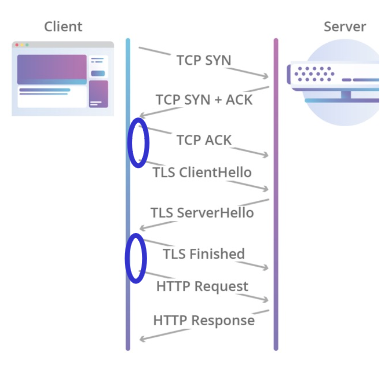
\includegraphics[scale=0.4]{images/tcp-n-tls.png}
\end{center}
\subsection*{Go-Back-N}
Sender has sliding window and can send many unacknowledged packets.
Acknowledgement is for the latest received packet w/o error and sender
window slides. On packet loss it retransmits all packets in the sliding
window. ACKs are cumulative. It does not buffers packets.
\subsection*{Selective Repeat}
Sender has sliding window and can send many unacknowledged packets.
Receiver acknowledges each received packet, and it buffers them
(out-of-order if necessary). Sender "selects" ACKed packets and re-sends
unACKed ones when their individual timers expire.